\documentclass[journal, a4paper]{IEEEtran}
\raggedbottom
\usepackage{fontspec}
\usepackage{polyglossia}
\setmainlanguage{spanish}
\setmainfont{Arial}
\usepackage{amsmath}
\usepackage{graphicx}
\usepackage{float}
\usepackage{booktabs}
\usepackage[hidelinks]{hyperref}
\graphicspath{{../assets/screens/}{../fixtures/}}

\title{Proyecto Final: Transformador de imágenes para contexto LLM}
\author{
Alejandro Apodaca Cordova, \textit{Matrícula: m041852}\\
Gael Calderon Robles, \textit{Matrícula: m042449}\\
Ingeniería Mecatrónica, CETYS Universidad, Campus Mexicali
}

\begin{document}
\maketitle

\begin{abstract}
En este proyecto se desarrolló un prototipo web de procesamiento digital de señales para convertir imágenes de entrada a JPG comprimido antes de subirlas a una aplicación de chat con modelos LLM. El sistema adquiere imágenes reales en el navegador, remuestrea su resolución, aplica una transformación opcional a luminancia, codifica la salida en JPEG y calcula métricas de ahorro y fidelidad. La herramienta permite justificar técnicamente cuántos recursos se reducen antes de enviar archivos a un servidor, usando bytes, expansión base64, error cuadrático medio y PSNR como indicadores.
\end{abstract}

\begin{IEEEkeywords}
procesamiento digital de imágenes, compresión JPEG, remuestreo, PSNR, aplicaciones LLM, herramientas web.
\end{IEEEkeywords}

\section{Introducción}
Las aplicaciones actuales de chat multimodal permiten adjuntar imágenes para análisis, soporte técnico o documentación. Sin embargo, las cámaras de teléfonos y computadoras generan archivos con resoluciones mayores a las necesarias para muchas consultas. Subir esas imágenes sin procesamiento previo aumenta el ancho de banda, el almacenamiento temporal, el tiempo de transferencia y el tamaño de los mensajes cuando la imagen se transforma a base64 para una API.

El problema de ingeniería consiste en reducir el costo de transmisión sin destruir la información visual que necesita el modelo. Para resolverlo se implementó una herramienta web que procesa la imagen localmente, antes de que llegue al servidor. La justificación principal es que una imagen digital es una señal discreta bidimensional; por lo tanto, su compresión puede estudiarse con fundamentos de procesamiento digital de señales: muestreo, cuantización, transformación de color, codificación con pérdida y medición de error.

\section{Marco teórico}
Una imagen digital puede representarse como una función discreta \(x[m,n]\), donde \(m\) y \(n\) son coordenadas espaciales y cada muestra contiene intensidad o color. Cuando se reduce la dimensión máxima de una imagen, se disminuye el número total de muestras. Este proceso es un remuestreo espacial y modifica directamente la cantidad de información que debe almacenarse o transmitirse.

La conversión opcional a luminancia usa el modelo perceptual:
\[
Y = 0.299R + 0.587G + 0.114B
\]
Con esto se conserva principalmente la información de brillo y se elimina la dependencia del color cuando la aplicación no lo requiere. Después se codifica la imagen en JPEG. Aunque el navegador abstrae internamente la transformada discreta del coseno y las tablas de cuantización, el parámetro de calidad controla la pérdida introducida por la cuantización.

Para evaluar la fidelidad, se compara la imagen remuestreada de referencia contra el JPEG decodificado. El error cuadrático medio se calcula como:
\[
MSE = \frac{1}{N}\sum_{i=1}^{N}(x_i-\hat{x}_i)^2
\]
y el PSNR como:
\[
PSNR = 10\log_{10}\left(\frac{255^2}{MSE}\right)
\]
Un PSNR mayor indica menor degradación numérica. En este proyecto no se interpreta solo: se combina con el ahorro de bytes, porque una compresión extrema puede ahorrar recursos pero perder detalles relevantes para el usuario o para el modelo.

\section{Enunciado del proyecto}
El proyecto final solicita desarrollar un sistema basado en técnicas de procesamiento digital de señales que permita adquirir, analizar, filtrar, transformar o interpretar señales reales utilizando herramientas computacionales y fundamentos teóricos de DSP. A partir de ese objetivo se planteó la siguiente aplicación: un transformador de imágenes para chats LLM que convierta varios formatos de imagen a JPG comprimido antes de subirlos a un servidor.

La herramienta busca responder tres preguntas de investigación:
\begin{enumerate}
\item ¿Cuánto peso se reduce al remuestrear una imagen y codificarla como JPEG?
\item ¿Qué costo aproximado se evita cuando una imagen se serializa en base64 para una aplicación web?
\item ¿Qué pérdida numérica introduce la compresión bajo una configuración dada?
\end{enumerate}

\section{Desarrollo}
El prototipo se implementó con Vite, React, TypeScript y Tailwind CSS para que sea publicable como página web estática. La cadena de procesamiento se ejecuta completamente en el navegador:
\begin{enumerate}
\item El usuario carga una o varias imágenes mediante selector o arrastre.
\item El navegador decodifica la imagen y registra tipo, resolución y bytes originales.
\item Se calcula una escala para limitar el lado mayor a una dimensión máxima configurable.
\item La imagen se dibuja en un \texttt{canvas}, lo cual realiza el remuestreo espacial.
\item Opcionalmente se aplica la transformación RGB a luminancia.
\item El \texttt{canvas} se codifica como \texttt{image/jpeg} con calidad configurable.
\item El JPG generado se decodifica otra vez para calcular MSE y PSNR contra la referencia.
\item La interfaz muestra ahorro de bytes, relación de compresión, ahorro base64 y descarga del JPG final.
\end{enumerate}

El modelo de ahorro considera que base64 expande el binario aproximadamente a \(4/3\). Para estimar unidades de contexto se divide el tamaño base64 entre cuatro caracteres por unidad. Esta aproximación no sustituye el conteo interno de ningún proveedor de LLM, pero sí sirve para comparar de forma reproducible la reducción relativa entre imagen original e imagen comprimida.

\begin{figure}[H]
\centering
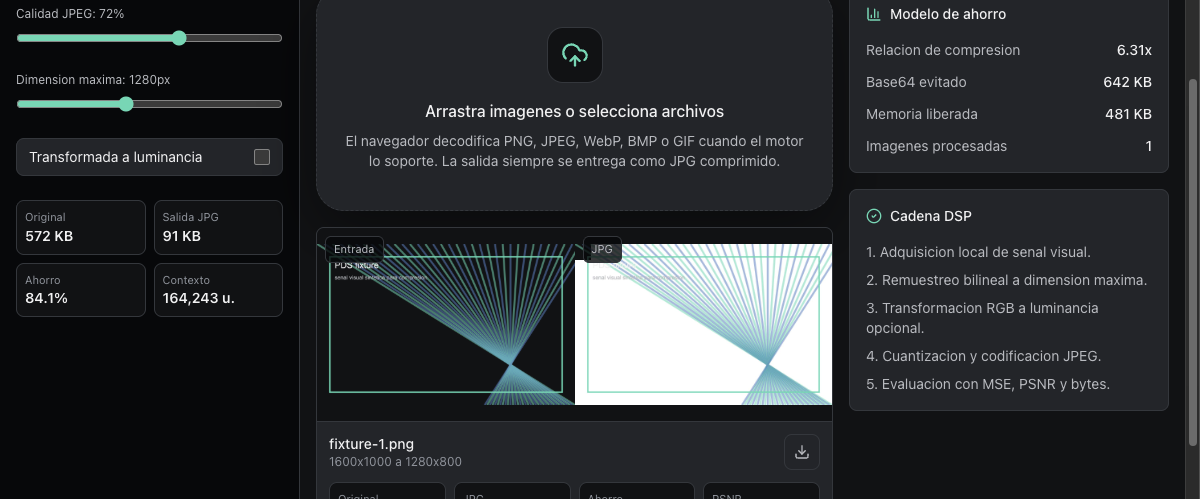
\includegraphics[width=\linewidth]{app_desktop.png}
\caption{Prototipo web ejecutado en escritorio con una imagen de prueba procesada.}
\end{figure}

\section{Resultados}
En la prueba reproducible con \texttt{fixture-1.png}, el sistema procesó una imagen de \(1600\times1000\) pixeles y la remuestreó a \(1280\times800\) pixeles usando calidad JPEG del 72\%. El archivo pasó de 572 KB a 91 KB, con ahorro de 84.1\%, relación de compresión de 6.31x y PSNR de 36.2 dB. Además, el modelo estimó 642 KB de base64 evitado y 164,243 unidades aproximadas de contexto ahorradas.

\begin{table}[H]
\centering
\caption{Resumen de la verificación del prototipo.}
\begin{tabular}{l c}
\toprule
Métrica & Resultado\\
\midrule
Tamaño original & 572 KB\\
Tamaño JPG & 91 KB\\
Ahorro directo & 84.1\%\\
Relación de compresión & 6.31x\\
Base64 evitado & 642 KB\\
PSNR & 36.2 dB\\
\bottomrule
\end{tabular}
\end{table}

También se revisó la interfaz en una vista móvil. Los controles principales permanecieron accesibles y las métricas se acomodaron en una cuadrícula de dos columnas, manteniendo el mismo estilo visual compacto usado en las prácticas previas: resultados visibles, explicación técnica breve y evidencia reproducible.

\begin{figure}[H]
\centering
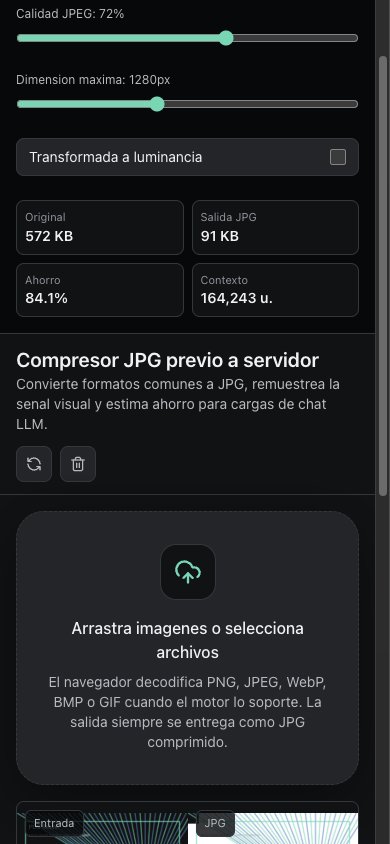
\includegraphics[width=0.48\linewidth]{app_mobile.png}
\caption{Verificación móvil de la herramienta.}
\end{figure}

\section{Alineación con 24ICE04 y 24ICE05}
Para 24ICE04, el proyecto identifica un problema de ingeniería concreto: el costo de subir imágenes sin optimización a chats LLM. La metodología incluye variables controlables, como calidad JPEG, dimensión máxima y luminancia, y variables de respuesta, como bytes comprimidos, PSNR y ahorro base64. El experimento permite analizar patrones y formular conclusiones sobre el balance entre fidelidad y recursos.

Para 24ICE05, el proyecto crea y aplica una herramienta moderna de ingeniería y TI. La selección de Vite, React, TypeScript y procesamiento en navegador se justifica porque permite publicar la solución en la web y evitar que imágenes pesadas lleguen al servidor antes de transformarse. Las limitaciones técnicas también se reconocen: JPEG no conserva transparencia, la compatibilidad de formatos depende del navegador y PSNR no garantiza por sí solo que un LLM interprete igual la imagen comprimida.

\section{Conclusión}
El prototipo demuestra que las técnicas de procesamiento digital de señales pueden aplicarse directamente a una necesidad actual de aplicaciones con IA. El sistema adquiere señales visuales reales, las transforma mediante remuestreo y codificación JPEG, analiza su error y cuantifica el ahorro de recursos. La configuración inicial recomendada es dimensión máxima de 1280 px y calidad JPEG entre 70\% y 80\%, porque en la prueba realizada produjo una reducción superior al 80\% con PSNR aceptable para contexto visual general.

Como mejora futura se puede agregar detección automática de texto pequeño, OCR de validación, comparación perceptual SSIM y pruebas directas con modelos multimodales para confirmar que la compresión no afecta la respuesta semántica del chat. Aun así, la herramienta ya cumple el objetivo de transformar imágenes antes de subirlas y ofrece métricas claras para tomar decisiones de ingeniería.

\onecolumn
\section{Código y repositorio}
El código fuente está organizado como una aplicación web publicable. Los módulos principales son:
\begin{itemize}
\item \texttt{src/App.tsx}: interfaz, controles y presentación de métricas.
\item \texttt{src/imageProcessing.ts}: remuestreo, luminancia, codificación JPEG, MSE y PSNR.
\item \texttt{src/metrics.ts}: cálculo de ahorro, base64 y unidades aproximadas de contexto.
\item \texttt{scripts/verify-metrics.mjs}: verificación reproducible del modelo de ahorro.
\end{itemize}

\begin{thebibliography}{9}
\bibitem{gonzalez} R. C. Gonzalez y R. E. Woods, \textit{Digital Image Processing}. Pearson.
\bibitem{oppenheim} A. V. Oppenheim y R. W. Schafer, \textit{Discrete-Time Signal Processing}. Pearson.
\bibitem{jpeg} G. K. Wallace, ``The JPEG Still Picture Compression Standard'', \textit{Communications of the ACM}.
\bibitem{mdncanvas} MDN Web Docs, \textit{Canvas API}.
\end{thebibliography}

\end{document}
